\subsubsection{ABI lower: lowering function call}
    
Procedure Call Conventions as follow:

Initialization points to the first address of frame stack after the \texttt{[fp]} register is loaded.
    
The address will be increased when the \texttt{[call]}  instruction is executed later. When the \texttt{[ret]} instruction is executed, the \texttt{[fp]} register points to the address and falls back.
    
    
the Calling Process is as follow:
\begin{itemize}
    \item call label

Use  \texttt{[call]} inst to call function as \texttt{[call functionLabel]}, and \texttt{[fp]} points to the new frame.\par
The \texttt{[pc]} address returned by the function is placed in \texttt{[fp-1]} which is detected by vm but not visiable by compiler backend.\par
insts pattern:
\begin{lstlisting}[language={}]
main:
.LBL0_0:
  ...
  call foo
  ...
foo:
.LBL1_0:
  ...
\end{lstlisting}
    \item function address

The address pointed to by fp before the function call is placed in  \texttt{[fp-2]} as \texttt{[mstore [r8,-2] r8]}.\par
insts pattern:
\begin{lstlisting}[language={}]
mstore [r8,-2] r8
\end{lstlisting}
    \item passing arguments

Function parameter processing: the first three input parameters are placed in the three registers \texttt{[r1]}, \texttt{[r2]}, and \texttt{[r3]}.
If there are more than 3 parameters, start with the fourth input parameter and descend accordingly in \texttt{[fp-3]} , \texttt{[fp-4]}, \texttt{[...]}. \par
insts pattern:
\begin{lstlisting}[language={}]
mov r1 vreg1
mload r2 [r8,offset]
mov r3 vreg2
\end{lstlisting}
    \item  local variables

Local variables inside the function start at \texttt{[fp]}, and the \texttt{[fp]} address is stored incrementally. 
\begin{lstlisting}[language={}]

The return value is stored in \texttt{[r0]}. If the return value is not a domain element, it needs to be returned by a memory pointer that returns the data.\par
insts pattern:
\begin{lstlisting}[language={}]
mov r0 vreg3
\end{lstlisting}
\end{itemize}

The call stack frames layout is as follows:

\begin{figure}[!htp]
    \centering
    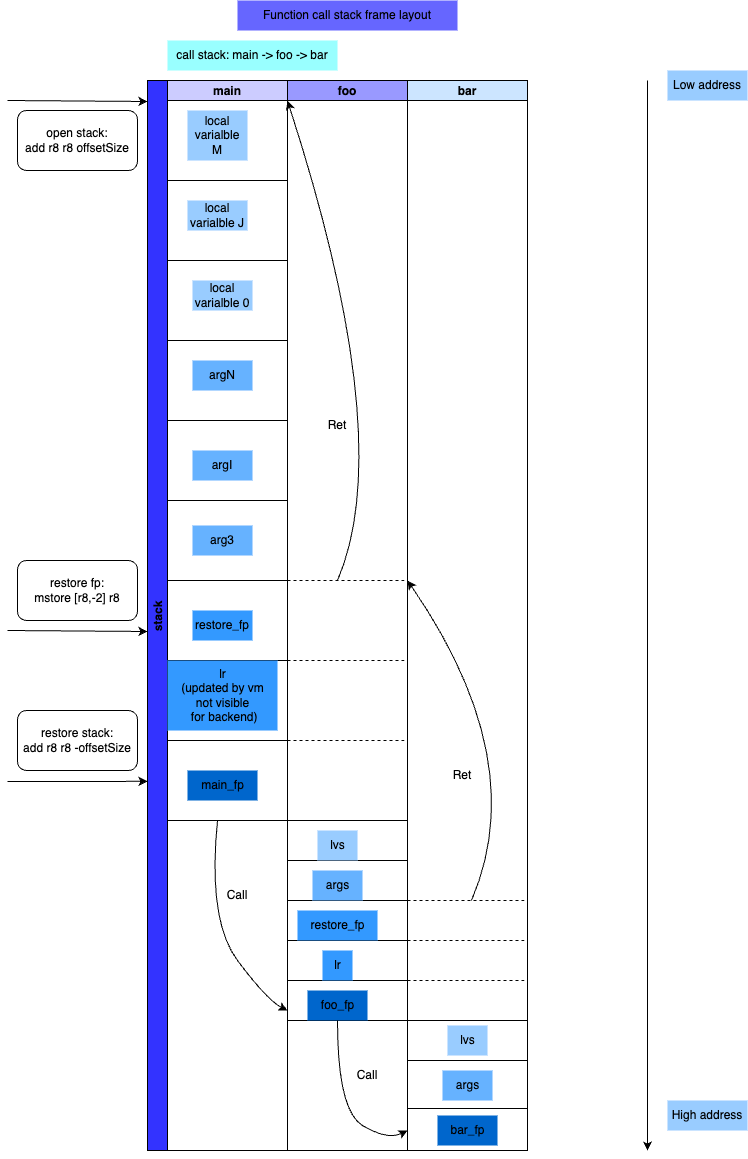
\includegraphics[width=0.6\textwidth]{ola-lang-backend-functioncall.jpg}
    \caption{Ola-lang functioncall layout}
    \label{fig:ola-lang-backend-functioncall}
\end{figure}

For prophet library functions, its insts pattern as:
\begin{lstlisting}[language={}]
.PROPHET{funcNum}_{prophetNum}:  // bind to prophet label
mov r0 psp  // interact with prophet readonly memory, get return value from prophet pointer
mload r0 [r0,0]  // used returned r0 as indexed addressing
\end{lstlisting}

First PROPHET label bind to prophet. Then interact with prophet readonly memory, get return value from prophet pointer \texttt{[psp]} to write into \texttt{[r0]}.
at last used it as indexed addressing to go on next program.